\section{Growth stages through late times}

\begin{figure*}
\begin{subfigure}[b]{\columnwidth}
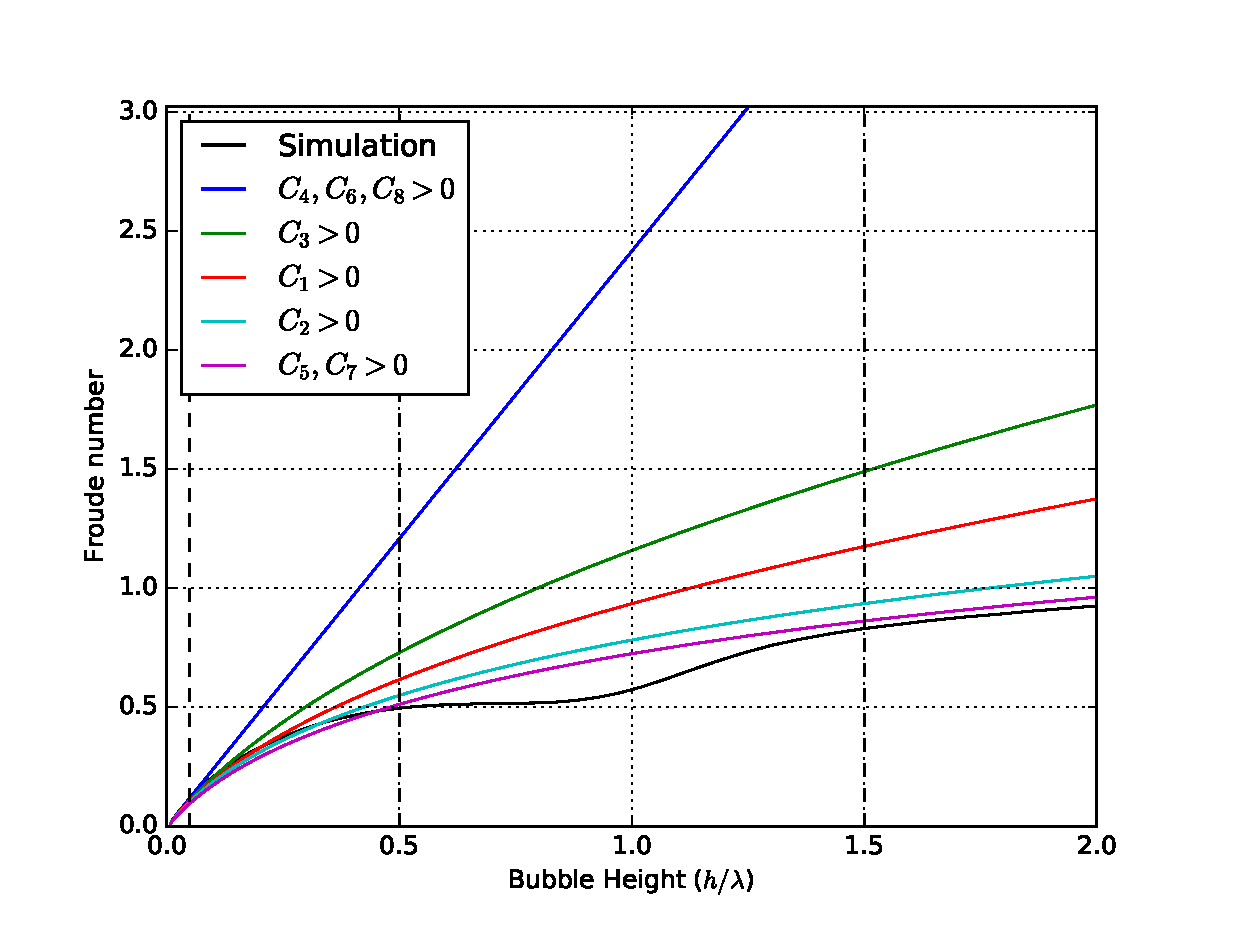
\includegraphics[width=\columnwidth]{figs/Cascade-short-4-1}
\caption{Early times}
\end{subfigure}
\begin{subfigure}[b]{\columnwidth}
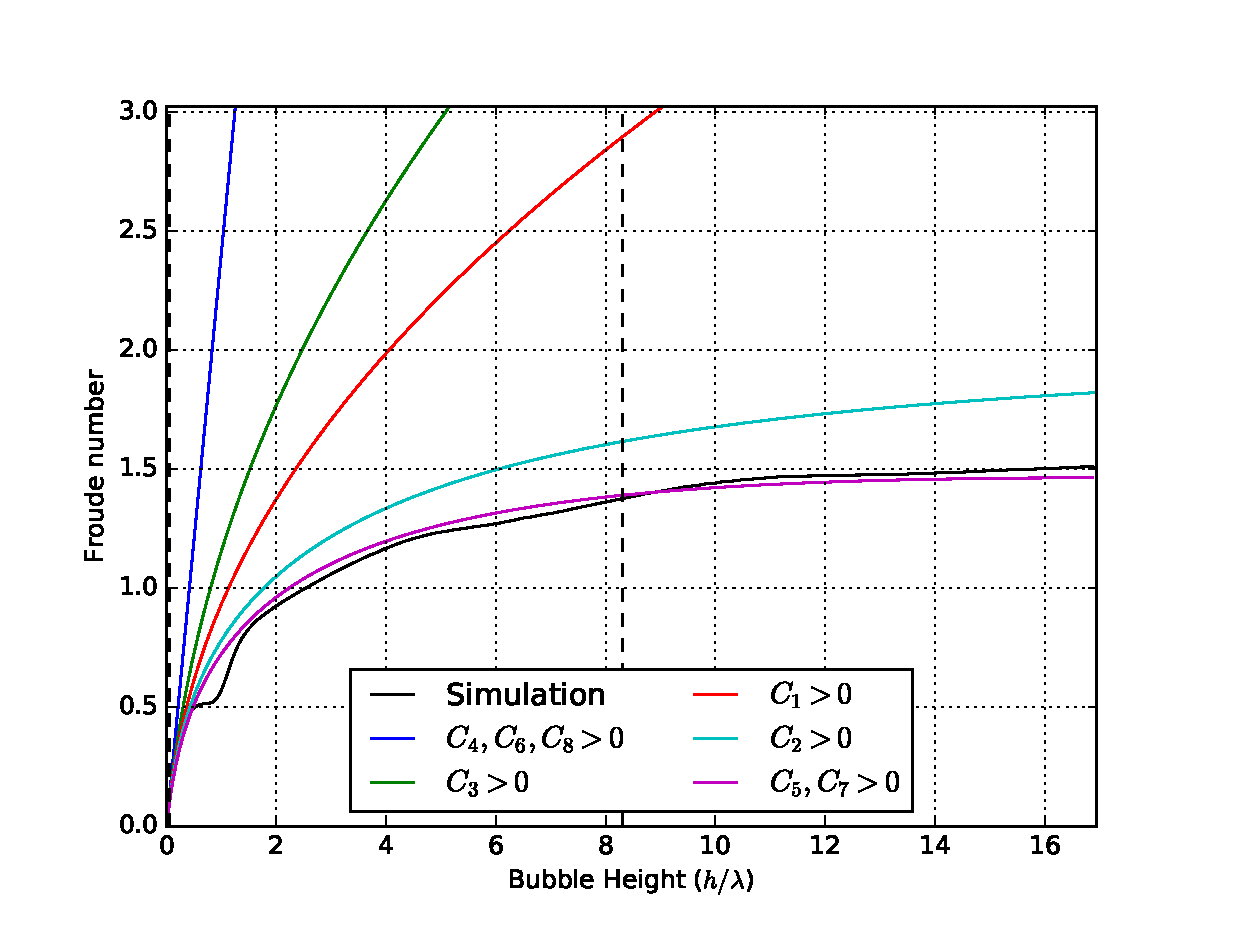
\includegraphics[width=\columnwidth]{figs/Cascade-4-1}
\caption{Late times}
\end{subfigure}
\caption{ \flabel{high_Ra_traj}
Bubble Froude number vs non-dimensional bubble height for $\text{Ra} = 10^{5.75}, \text{Sc} = 4$, simulation vs model with succesive terms enabled.
The dashed vertical lines divide the trajectory into four regimes: linear growth for $H/\lambda < .05$, saturation until $H / \lambda = 0.5$, stagnation and reacceleration until $H / \lambda = 1.5$, and dissipation beyond that.
}
\end{figure*}

\begin{figure*}
\begin{subfigure}[b]{\columnwidth}
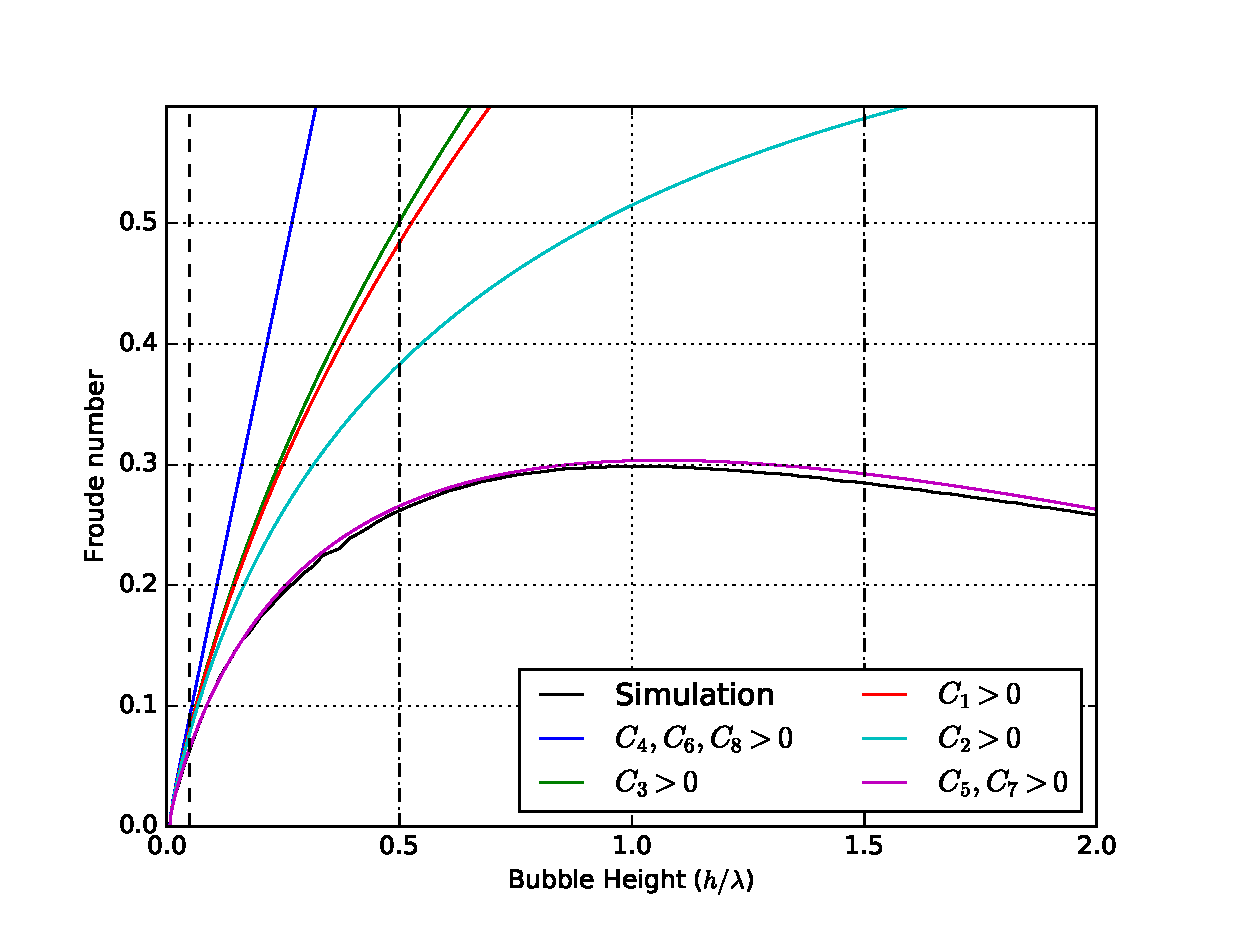
\includegraphics[width=\columnwidth]{figs/Cascade-short-32-4}
\caption{Early times}
\end{subfigure}
\begin{subfigure}[b]{\columnwidth}
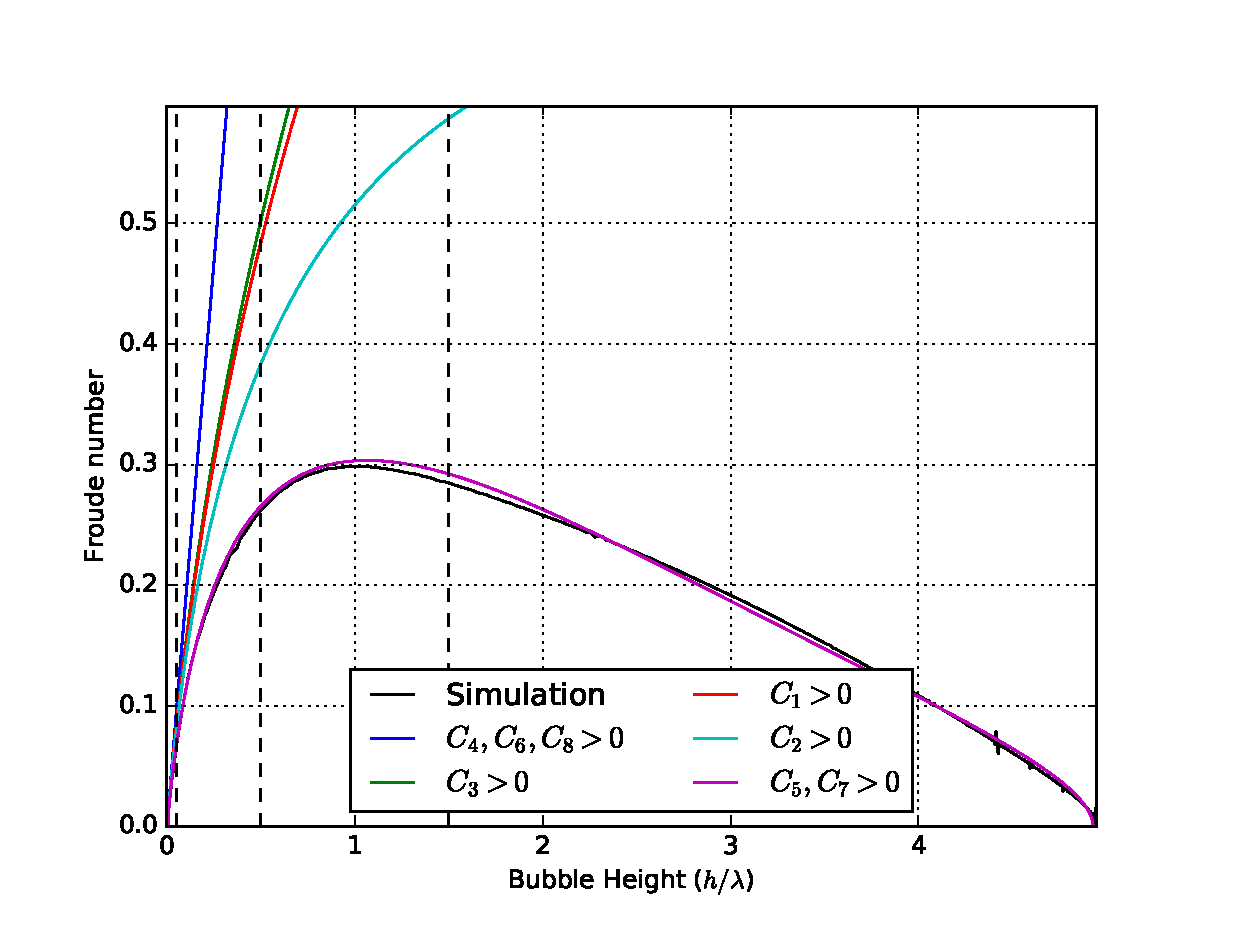
\includegraphics[width=\columnwidth]{figs/Cascade-32-4}
\caption{Late times}
\end{subfigure}
\caption{ \flabel{low_Ra_traj}
Bubble Froude number vs non-dimensional bubble height for $\text{Ra} = 10^{4.5}, \text{Sc} = 8$, simulation vs model with succesive terms enabled.
Dashed vertical lines divide the trjaectory, as in \fref{high_Ra_traj}, but the saturation regime and stagnation and reacceleration regime are surpressed by mixing.
}
\end{figure*}

In the spirit of recent analyses~\cite{Ramaprabhu2012, Wei2012}, we try to identify growth stages.
To do so, we consider the behavior of the simple model with coefficients set to zero.
Initially, only $C_4$, $C_6$, and $C_8$ affect bubble dynamics.
The growth is exponential with a rate in agreement with the linear theory, so we term this the linear regime.
As the bubble grows, the $C_3$ term reduces the growth rate to a limiting value of $A g / C_3$.
Because this represents the transition from exponential growth to free-fall, we term it the saturation regime.
The $C_1$ term has the same qualitative effect as the $C_3$ term, so it doesn't distinguish a unique regime.
The $C_2$ term does impose a limiting velocity scale, so it departs significantly from the $C_3$ dynamics in the viscous regime.
Finally, the $C_5$ term, balanced by the $C_7$ term, mix the fluid and reduce the effective Atwood number in the diffusive regime.
Because the relative onset of the viscous and diffusive regimes depends on the Schmidt number, they are grouped together into the dissipative regime.
Ultimately, the bubble stops rising.
The bubble height at this point, which is also the maximum bubble height, is called the penetration depth.

\subsection{Expoential growth}
When the amplitude is small and the interface is thin, the linear theory and numerical results identify exponential growth: $\ddot{h} = \gamma^2 h$.
Similarly, in the limit $h, \delta \rightarrow 0$, the simple model yields a growth rate:
\begin{equation}
\gamma = \sqrt{\frac{A_0 g k}{2 \pi C_4(1 + C_8 / C_6 \pi^{1/2} k \delta)}},
\end{equation}
which differs from the linear theory by the absence of a $-D k^2$ term.
This is the only term that can cause unstable interfaces to decay, i.e. $\gamma < 0$ for positive Atwood numbers.
In the simple model, all unmixed bubbles grow while in the lineary theory highly diffusive bubbles decay.

The other terms scaled by the other coefficients, i.e. $C_1, C_2, C_3, C_5, C_7$, can be omitted while the description of the exponential growth is unaffected.

\subsection{Saturation}
The exponential growth saturates as the bubble height increases.
In the simple model, this captured by the $C_3$ term:
\begin{equation}
\ddot{h} = \frac{A g}{(C_3 h + C_4 \lambda) (1 + C_8 / C_6 \pi^{1/2} k \delta)},
\end{equation}
which becomes significant when $h \approx C_4 \lambda / C_3$.
We will find in the following section that $C_3$ takes a value of about 1, so, omitting viscous corrections, saturation halves the growth rate at $h \approx \lambda / (2\pi)$.

\subsection{Stagnation and reacceleration}

For sufficiently high Grashof numbers, the saturation regime is followed by a stagnation of the velocity, itself followed by a re-acceleration, as seen in \fref{high_Ra_traj}.
There are no terms in the buoyancy-drag model capable of producing an inflection point in the Froude number vs bubble height, so stagnation and reacceleration cannot be controlled by turning a model coefficient on or off.
This suggests that the buoyancy-drag model is missing a term.

As the height grows, the $C_2$ term does impose a limiting velocity, \eref{visc_vel}.
When this limiting velocity is near or below the stagnation velocity, $\text{Fr} \approx \pi^{-1/2}$, saturation and reacceleration are surpressed.


\subsection{Dissipative regime}

As the bubble height increases, so does the surface area of the bubble.
When the viscous drag reduces the bubble's acceleration, the flux of pure fluid into the bubble, which goes as the velocity, is unable to math the flux of mixed fluid through the interface.

Beyond the stagntion and reacceleration regime, if present, late time mixing continues to influence the trajectory.
The sidewall mixing term scaled by $C_5$ and bubble volume term scaled by $C_7$ are essential to the flow.
Conversely, the high Rayleigh number trajectories that are clipped when they interact with the top wall underscontrain $C_5$ and $C_7$.
This will later motivate the addtion of a regularization term to the fit.

\subsection{Penetration depth}

The penetration depth is the maximum height of the bubble, which is the height of the bubble at the stopping condition of this analysis.
We can estimate the scaling of the penetration depth as the product of a characteristic velocity with a characteristic time-scale.
The late-time velocity is given by viscosity:
\begin{equation}
v_\nu \sim \frac{ A g \lambda^2}{\nu},
\end{equation}
while time-scale is given by diffusion:
\begin{equation}
\tau_D = \frac{\lambda^2}{D}.
\end{equation}
Combining and non-dimensionalizing by the wave-length yeilds:
\begin{equation}
\frac{h(\infty)}{\lambda} = \frac{A g \lambda^3}{\nu D} = \text{Ra},
\end{equation}
so the penetration depth should go linearly with the Rayleigh number.

The penetration depth is plotted as a function of Rayleigh and Schmidt number in \fref{depth_scatter}, and, indeed, depends strongly on the Rayleigh number before being clipped by the top walls.
Furthermore, the relationship to the Rayleigh number is linear over the cases shown here, as shown in \fref{depth_line}.

